\begin{fex}
 Soit l'application $f \colon z \mapsto \exp\left(i z^2\right)$. 
\begin{enumerate}
  \item Montrer que $f$ est holomorphe sur $\mathbb{C}$ et vérifier que sa
  dérivée est continue.
  \item Pour tout réel $r > 0$, le contour $\gamma_r$ est défini selon la figure
  \ref{fig:contour2}. Donner la valeur de l'intégrale:
  \[
  \int_{\gamma_r} f(z) dz
  \]
  \item Ecrire cette intégrale sous la forme d'une somme de trois
  intégrales de chemin et montrer que l'intégrale correspondant à l'arc de
  cercle tend vers 0 lorsque $r \to +\infty$.
  \item En déduire les valeurs des intégrales généralisées suivantes, dites
  intégrales de Fresnel:
  \[
  \lim_{r \to +\infty} \int_{[-r,r]} \cos(x^2) dx, \quad  \lim_{r \to +\infty}
  \int_{[-r,r]} \sin(x^2) dx
  \]
\end{enumerate}
\end{fex}
 \begin{figure}[ht]
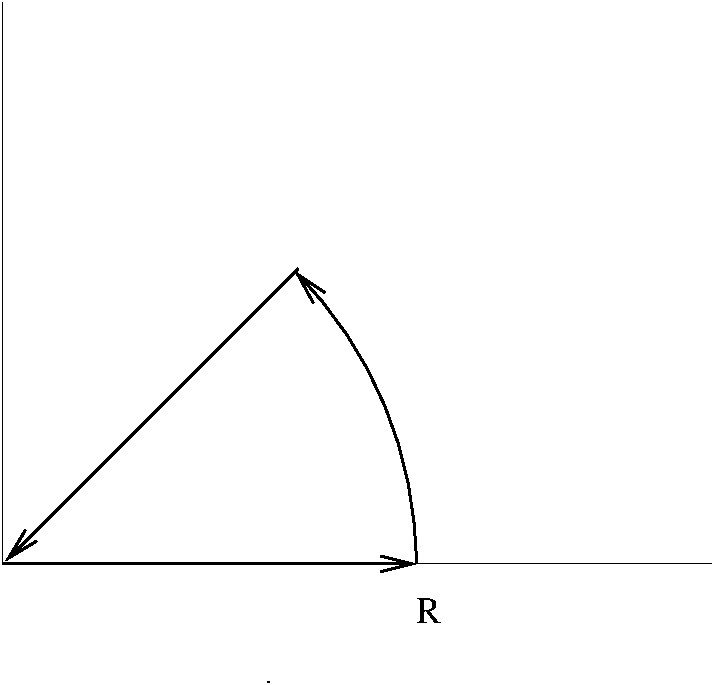
\includegraphics[scale=0.3]{contour_fresnel.pdf}
\caption{Contour $\gamma_r$}\label{fig:contour2}
\end{figure}
\begin{enumerate}
\item L'application $f$ est holomorphe comme composée d'applications
holomorphes. Sa dérivée est $f^\prime(z) = 2 i z f(z)$, qui est continue. 
\item
Par la formule de Cauchy, on a~:
\[
\int_{\gamma_3 . \gamma_2 . \gamma_1} f(z) dz = 0
\]
Par ailleurs~:
\[
\int_{[0,R]} e^{ix^2}d \lambda(x) = \int_{\gamma_1} f(z) dz
\]
En choisissant pour $\gamma_2$ le paramètrage~:
\[
t \in [0, \frac{\pi}{4}] \to \gamma_2(t) = R e^{it}
\]
on obtient~:
\[
\int_{\gamma_2} f(z) dz = \int_{[0, \frac{\pi}{4}]} e^{-R^2 \sin (2t)
+ i R^2 \cos(2t)} i R e^{it} d \lambda(t)
\]
On peut majorer le module de $\int_{\gamma_2} f(z) dz$ par~:
\[
\int_{[0, \frac{\pi}{4}]} e^{-R^2 \sin (2t)}  R d \lambda(t)
\]
Comme l'application $\sin$ est concave sur $[0, \frac{\pi}{2}]$, sur
cet intervalle on a~: $\sin(t) \geq \frac{2 t}{\pi}$, ce qui donne la
majoration~:
\[
\left | \int_{\gamma_2} f(z) dz \right | \leq 
\int_{[0, \frac{\pi}{4}]} e^{-\frac{R^2 4 t}{\pi}} R dt =
\frac{(\pi)(1- e^{-R^2})}{4 R}
\]
\item
\[
\int_{\gamma_3} f(z) dz = e^{i \frac{\pi}{4}} \int_{[0,R]} e^{-t^2} d\lambda(t)
\]
d'où en passant à la limite et en remarquant que $\lim_{R \to
+\infty}\int_{\gamma_2} f(z) dz = 0$~:
\[
I = J = \frac{1}{2} \sqrt{\frac{\pi}{2}}
\]
\end{enumerate}
\begin{fex}
 Soit $f \colon z \in \mathbb{C} \mapsto \exp(-z^2)$.
\begin{enumerate}
  \item Montrer que $f$ est holomorphe dans $\mathbb{C}$, de dérivée continue.
  \item En utilisant le contour $\gamma_r$ donné figure \ref{fig:contour3},
déterminer, pour
  $\omega \in \mathbb{R}$ fixé, la valeur de l'intégrale:
  \[
  \int_{\gamma_r} \exp(-z^2)dz
  \]
  \item En faisant tendre $r$ vers $+\infty$ et en faisant un raisonnement
  similaire à celui de l'exercice précédent, déterminer la transformée de
  Fourier de l'application $x \mapsto \exp(-x^2)$.
\end{enumerate}
\end{fex}
 \begin{figure}[ht]
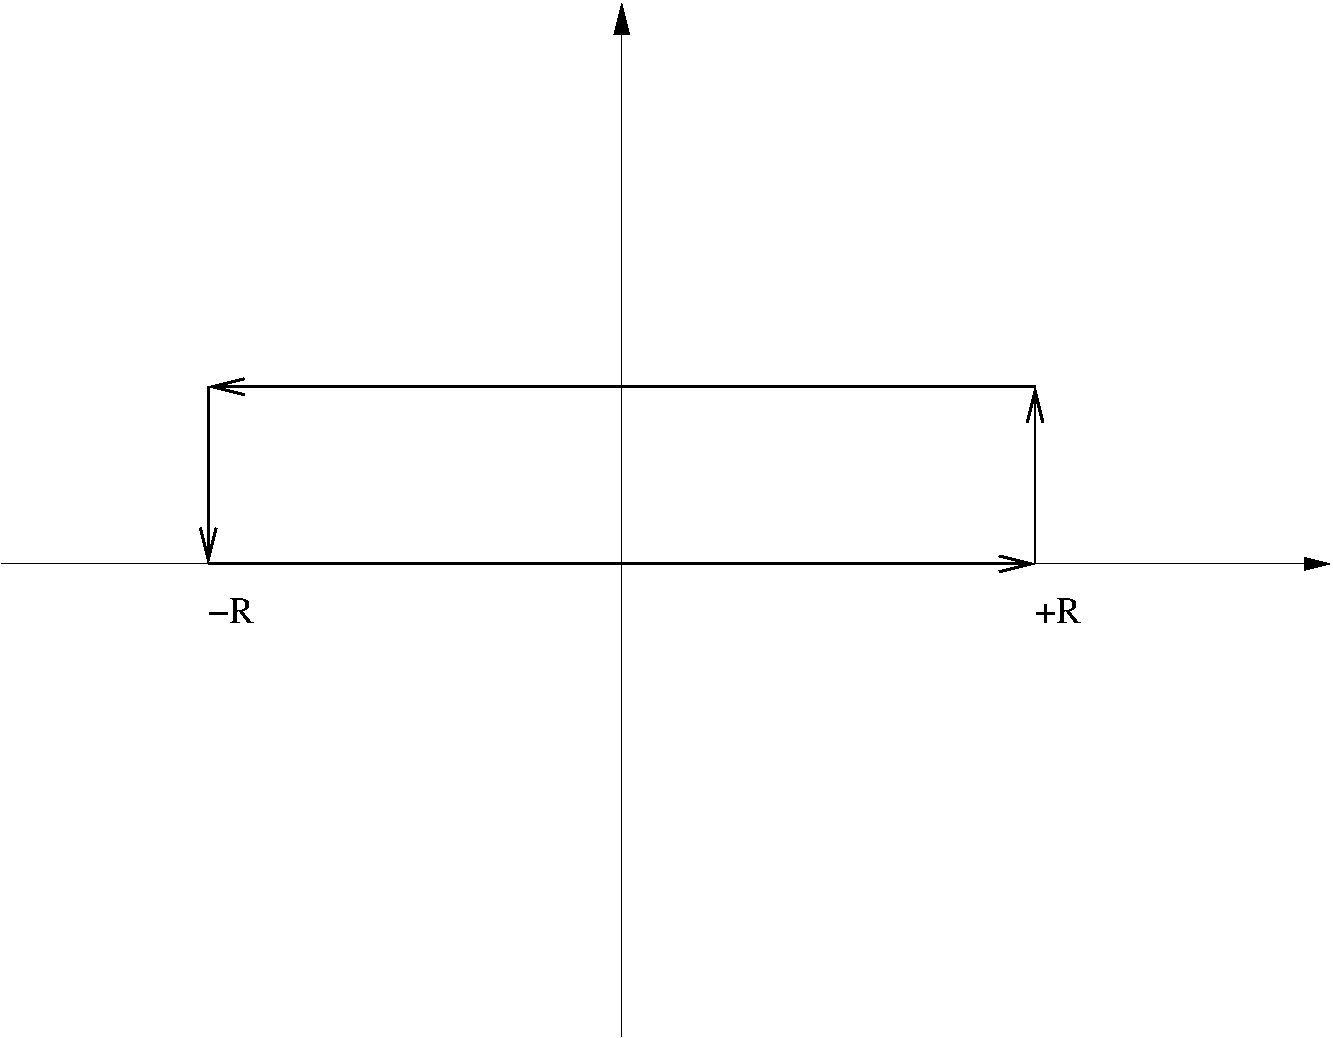
\includegraphics[scale=0.3]{contour_gauss.pdf}
\caption{Contour $\gamma_r$}\label{fig:contour3}
\end{figure}
\begin{enumerate}
 \item Même raisonnement que dans l'exercice précédent.
\item L'application intégrée est holomorphe, la formule de Cauchy s'applique:
\[
  \int_{\gamma_r} \exp(-z^2)dz = 0
  \]
\item L'intégrale sur l'axe réel est:
\[
 \int_{[-r,r]} \exp(-x^2) dx 
\]
de limite $\sqrt{\pi}$ pour $r \to +\infty$. Le segment supérieur se paramètre
par:
\[
 t \in [-r,r] \mapsto -t+i \frac{\omega}{2}
\]
L'intégrale le long de ce chemin est donc:
\[
 - \int_{[-r,r]} e^{-t^2 + i t \omega + \frac{\omega^2}{4}} dt
\]
La limite lorsque $r\to +\infty$ est:
\[
- e^{\frac{\omega^2}{4}} \int_\R  e^{-t^2 + i t \omega} dt 
\]

Finalement, l'intégrale sur les segments verticaux aura pour limite $0$ si $r
\to +\infty$. Un paramétrage possible du segment situé en $r$ est:
\[
t \in [0, \frac{\omega}{2}] \mapsto r + it 
\]
conduisant à l'intégrale:
\[
 i \int_{[0, \frac{\omega}{2}]} e^{-(r+it)^2} dt 
\]
son module se majore par:
\[
 \frac{\omega}{2}e^{-r^2 + \frac{\omega^2}{4}}
\]
qui a bien pour limite $0$ lorsque $r \to +\infty$. Le second segment vertical
se traite de la même façon. En regroupant les termes et en remarquant que la
transformée de Fourier est une application paire, on en déduit finalement
qu'il s'agit de l'application:
\[
 \omega \mapsto \sqrt{\pi} e^{-\frac{\omega^2}{4}}
\]
\end{enumerate}